% % % % % % % % % % % % % % % % % % % % % % % % %
\chapter{4-manifolds}
% % % % % % % % % % % % % % % % % % % % % % % % %

% ----------------------
\section{Bordism}
% ----------------------

\begin{definition}
	The $n$-dimensional oriented \textit{cobordism group}
	\index{cobordism group}
	over the space $X$ is
	\begin{equation*}
		\Omega_{n}[X] =
			\frac{ \{ f \colon M^{n} \rightarrow X \mid M^n \textrm{ oriented, closed, } 
			n\textrm{-dim. manifold} \}}{\textrm{bordism}}
	\end{equation*}
	\marginnote{If $\alpha \colon M^{n} \rightarrow X$
		represents a bordism class, $M^n$ is allowed to
		have more than one component.}
\end{definition}

\begin{proposition}[{\citep[13.15, p. 319]{kauffman1987knots}}]
	\begin{itemize}
		\item Pushing forward a fundamental class
		\begin{align*}
			\Omega_n [X] & \rightarrow H_{n}(X ; \Z) \\ 
			[f \colon M^{n} \rightarrow X] & \mapsto f_{*}([M])
		\end{align*}
		is an isomorphism for $n \le 3$.
		
		\item The sequence
		\begin{equation*}
			\Omega_{4}[\ast] \rightarrow \Omega_{4}[X] \rightarrow H_{4}(X ; \Z)
		\end{equation*}
		is exact.
	\end{itemize}
\end{proposition}

%TODO

% ----------------------
\section{Andrews-Curtis Conjecture}
% ----------------------

\citep{SCP4}

\begin{definition}
	A \textit{balanced presentation} \index{presentation!balanced} is a presentation
	\[
		\langle g_1, \ldots, g_n \mid r_1, \ldots, r_n \rangle
	\]
	with the same number of generators and relations.
	
	The Andrew-Curtis moves on a balanced presentation are
	\begin{enumerate}[label=(\roman*)]
		\item \textbf{1-handle slides:} Replace a pair of generators
		$ \{ x, y \} $ by $ \{ x, xy \} $
		
		\item \textbf{2-handle slides:} Replace a pair of relations
		$ \{ r, s \} $ by $ \{ grg^{-1}s, s \} $, where $ g $ is any word in the generators
		
		\item \textbf{1-2-handle cancellations:} Add a generator together with
		a new relation killing it
	\end{enumerate}
	In particular, you are \underline{not} allowed to make a copy of a relation to
	keep for later use (which would correspond to 
	\textbf{2-3-handle creation/cancellation}).
\end{definition}

\begin{conjecture*}[Andrews-Curtis conjecture \textcolor{red}{(False?)}]
	Any balanced presentation of the trivial group can be transformed
	by Andrews-Curtis moves to the trivial presentation.
\end{conjecture*}

\begin{example}
	%TODO
	TODO
	\[
		\langle x, y \mid xyx = yxy, x^{5} = y^{4} \rangle
	\]
	is a balanced presentation of the trivial group,
	but until now nobody was able to find a sequence of
	Andrews-Curtis moves to transform it into the trivial presentation
	\[
		\langle x, y \mid x, y \rangle
	\]
\end{example}

%TODO
TODO
Explain how to construct homotopy $4$-spheres from balanced
presentations of the trivial group
\citep{akbulut1985potential}

% ----------------------
\section{Trisections}
% ----------------------

\begin{center}
	\textsc{``Trisections are to $4$-manifolds as Heegaard splittings are to
		$3$-manifolds''}
\end{center}

\subsection{References}

\begin{itemize}
	\item Original paper: \citep{gay2016trisecting}
	\item Lecture notes: \citep{gay2019heegaard}
\end{itemize}

\subsection{Definitions}

\marginnote{
	\begin{itemize}
		\item $\#^n A$ is the connected sum of $n$ copies of $A$,
		with $\#^{0} A = \sphere{m}$
		
		\item TODO
		%TODO
	\end{itemize}}
\begin{definition}
	\begin{itemize}
		\item The standard genus $g$ surface is
		\[
			\Sigma_g = {\#}^{g} (\sphere{1} \times \sphere{1})
		\]
		\item The standard genus $g$ solid handlebody is
		\[
			H_g = \natural^g (\sphere{1} \times \disk{2})
		\]
		with $\partial H_{g} = \Sigma_{g}$
		\marginnote{$\partial (A \natural B) = (\partial A) \# (\partial B)$}
		
		\item The standard $4$-dimensional $1$-handlebody
		(of ``genus $k$'') is
		\[
			Z_{k} =\natural^{k} (\sphere{1} \times \disk{3})
		\]
		i.e.\ a $4$-ball to which we attach $k$-many
		$4$-dimensional $1$-handles.
	\end{itemize}
\end{definition}
\begin{marginfigure}
	\begin{center}
		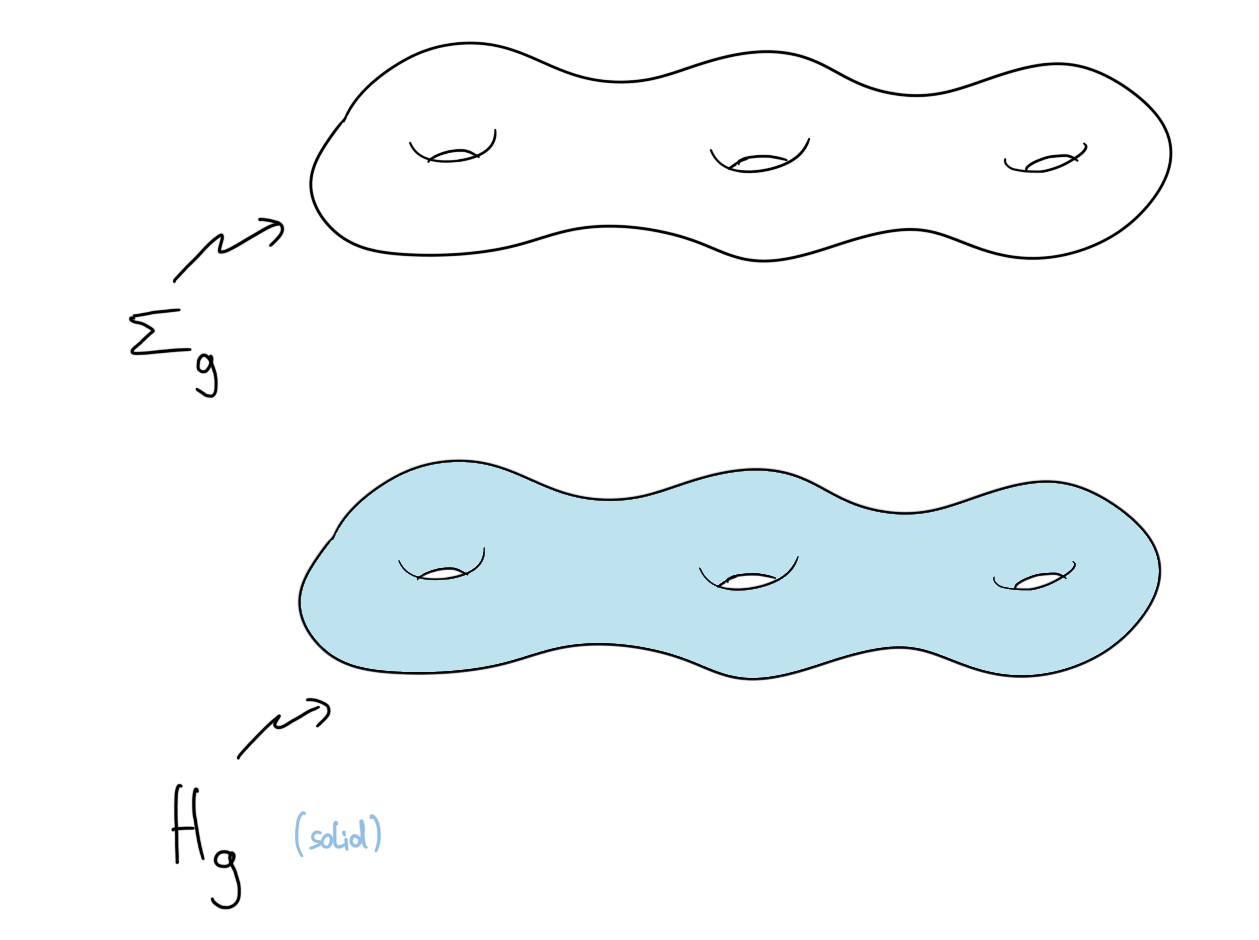
\includegraphics{./pictures/standard_manifolds.png}
	\end{center}
	\caption{Standard manifolds of dimension 2, 3}
	\label{fig:standard_manifolds}
\end{marginfigure}